\documentclass{article}
\usepackage[utf8]{inputenc}
\usepackage{listings}
\usepackage[english]{babel}
\usepackage{float}
\usepackage{caption}
\usepackage{courier}
\usepackage{graphicx}
\usepackage{mathtools}
\usepackage{subcaption}
\usepackage[bottom]{footmisc}
\usepackage{listings}
\graphicspath{{./images/}}


\title{CSN Lab 7 \\ Simulation of SIS model over networks}
\author{Juan Pablo Royo \& Francesc Roy}
\date{December 2020}

\usepackage{natbib}
\usepackage{graphicx}

\begin{document}

\maketitle

%%%%%%%%%%%%%%%%%%%%%%%%%%%%%%%%%%%%%%%%%%
%%%%%%%%%%% INTRODUCTION %%%%%%%%%%%%%%%%%
%%%%%%%%%%%%%%%%%%%%%%%%%%%%%%%%%%%%%%%%%%

\section{Introduction}

\noindent In this laboratory session we are going to simulate how and infection is spread over different networks following the SIS model.\\

\noindent We are going to play with different values of $\gamma$ (recovery probability of an infected node at each time step) and $\beta$ (probability to infect each neighbour if you are infected at each time step) and check how the epidemic evolve over time.\\

\noindent We are also going to play with the initial proportion of infected nodes $p_{0}$.\\

\noindent The networks for every set of initial conditions ($\gamma$, $\beta$, $p_{0}$) used will be: 

\begin{itemize}
  \item Fully connected network (complete graph)
  \item Scale-free network of Barabasi-Albert
  \item Small-world network of Watts-Strogatz
  \item Trees
  \item Star Network
  \item Regular lattices
  \item Erdos-Renyi random graphs\\
\end{itemize}









\newpage
\section{Tasks}
\subsection{Task 1}

\noindent In this task we are going to analyze how the epidemic occurs for a fixed set of $\beta$,$\gamma$ and $p_{0}$ values. All experiments are executed for 300 units of time which seems to be sufficient to reach an stable point to do the analysis.\\

\noindent SCENARIO 1: $\beta = 0.2$,$\gamma = 0.8$ and $p_{0} = 0.05$: \\

\noindent In this setup we can see there are networks (tree and Barabasi-Albert) where the epidemic drops very quickly to zero and never grows above the initial $p_{0}$.\\

\noindent On the other hand there are networks like Watts Strogatz and Erdos Renyi that stabilize the epidemic at some point around 60\% of infected people.\\

\noindent The fraction of infected people in the star network has a lot of variability but it also seems to be stabilized at around 0.15.\\

\begin{center}
   
    
    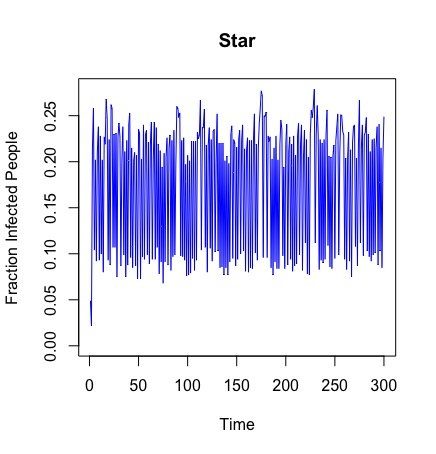
\includegraphics[width=6cm]{star.jpeg}
    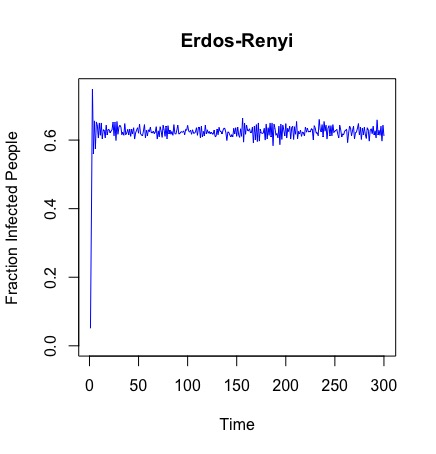
\includegraphics[width=6cm]{erdos_renyi.jpeg}
    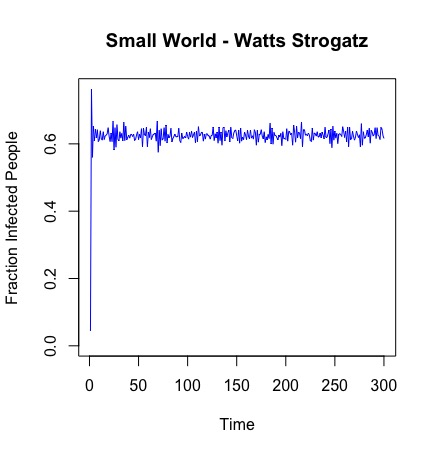
\includegraphics[width=6cm]{watts_strogatz.jpeg}
    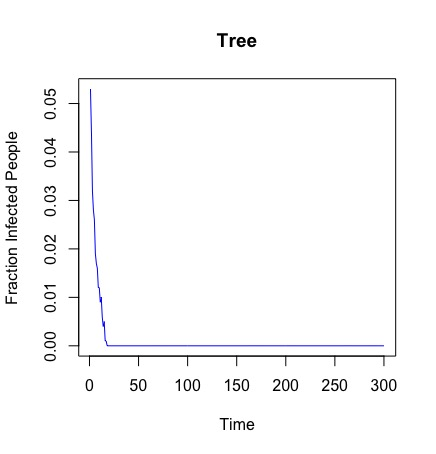
\includegraphics[width=6cm]{tree.jpeg}
    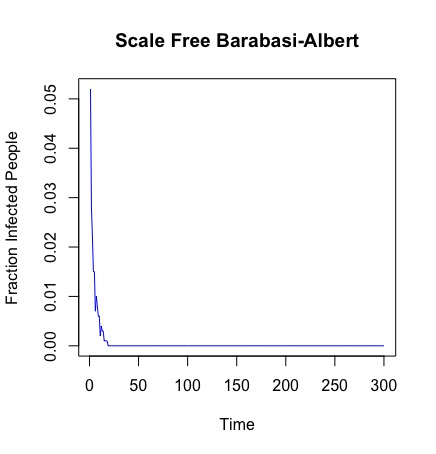
\includegraphics[width=6cm]{barabasi_albert.jpeg}
    
\end{center}


\newpage
\noindent SCENARIO 2: $\beta = 0.8$,$\gamma = 0.2$ and $p_{0} = 0.05$: \\

\noindent In this setup it seems that all networks are equally prone to spread the infection up to the 80\% of infected people. Its true that in Tree and Barabasi Albert networks it takes a little bit more time to reach this point.\\



\begin{center}
   
    
    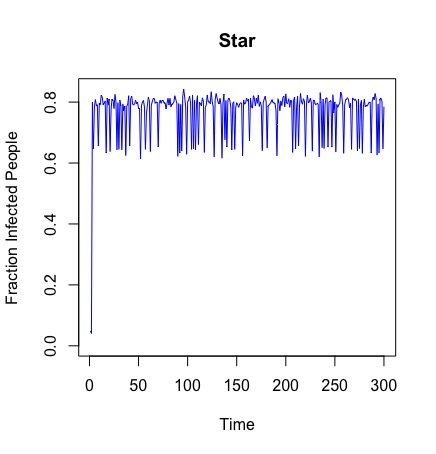
\includegraphics[width=6cm]{star_2.jpeg}
    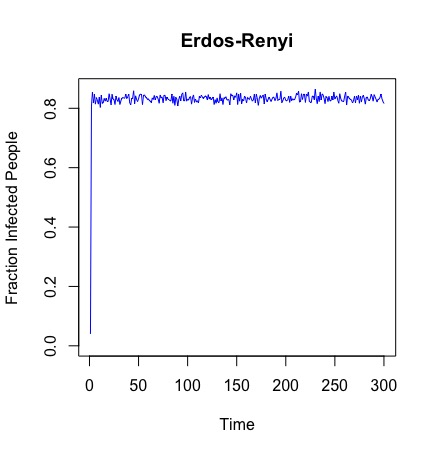
\includegraphics[width=6cm]{erdos_renyi_2.jpeg}
    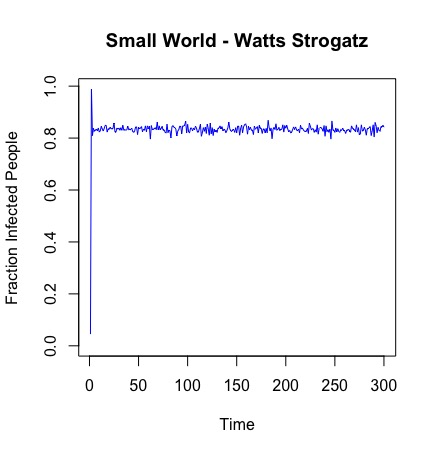
\includegraphics[width=6cm]{watts_strogatz_2.jpeg}
    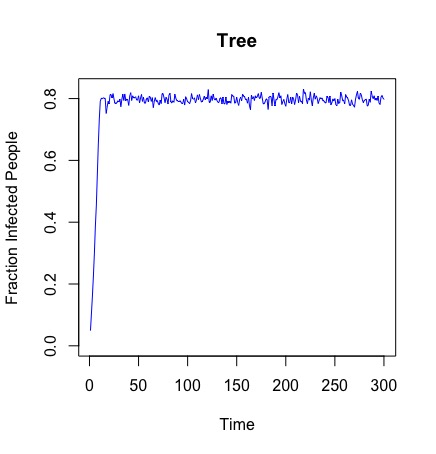
\includegraphics[width=6cm]{tree_2.jpeg}
    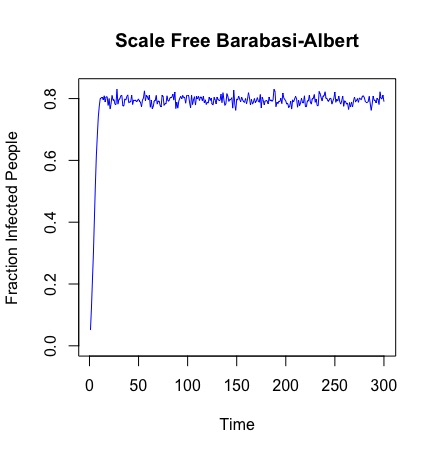
\includegraphics[width=6cm]{barabasi_albert_2.jpeg}
    
\end{center}

\newpage
\noindent SCENARIO 3: For $\beta = 0.2$,$\gamma = 0.8$ and $p_{0} = 0.3$: \\

\noindent Very similar to escenario 1.\\ 


\begin{center}
   
    
    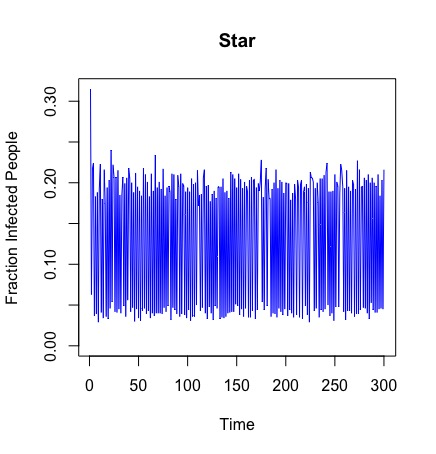
\includegraphics[width=6cm]{star_3.jpeg}
    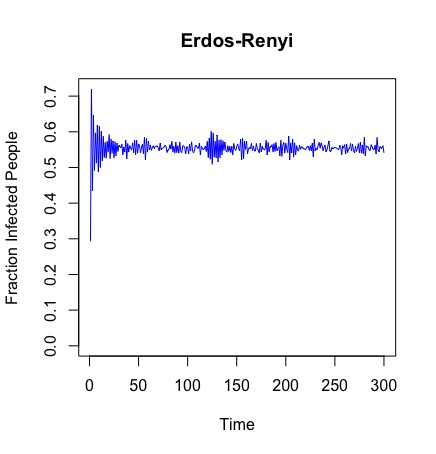
\includegraphics[width=6cm]{erdos_renyi_3.jpeg}
    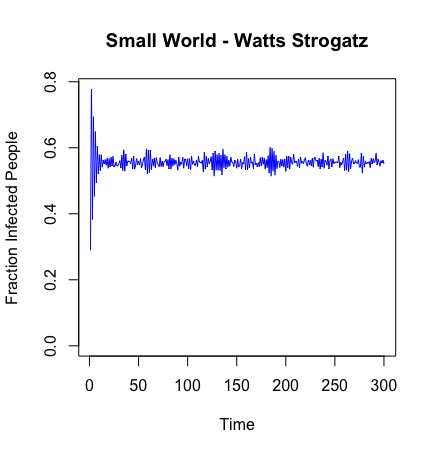
\includegraphics[width=6cm]{watts_strogatz_3.jpeg}
    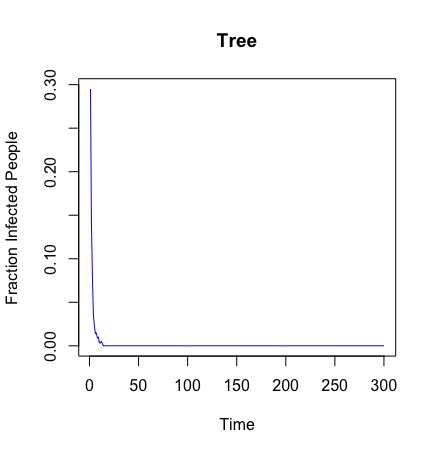
\includegraphics[width=6cm]{tree_3.jpeg}
    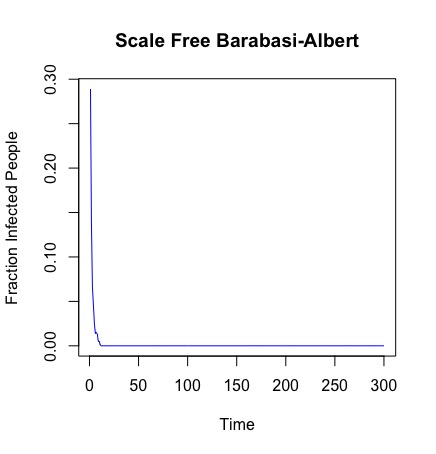
\includegraphics[width=6cm]{barabasi_albert_3.jpeg}
    
\end{center}

\newpage

\noindent SCENARIO 4: $\beta = 0.8$,$\gamma = 0.2$ and $p_{0} = 0.3$: \\

\noindent Very similar to escenario 2.\\

\begin{center}
   
    
    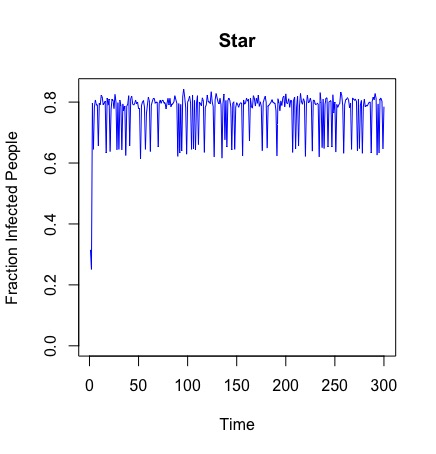
\includegraphics[width=6cm]{star_4.jpeg}
    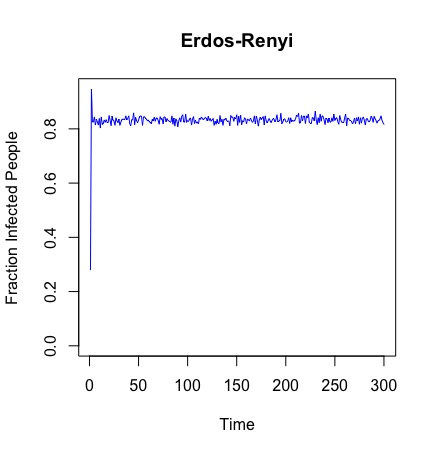
\includegraphics[width=6cm]{erdos_renyi_4.jpeg}
    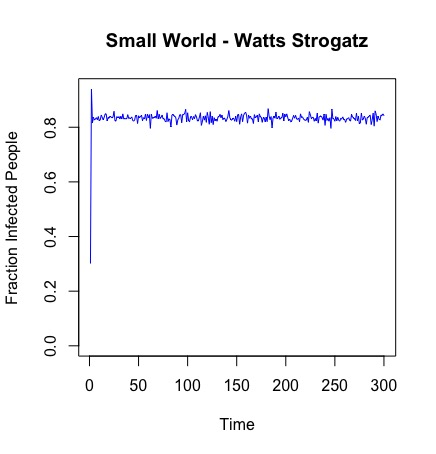
\includegraphics[width=6cm]{watts_strogatz_4.jpeg}
    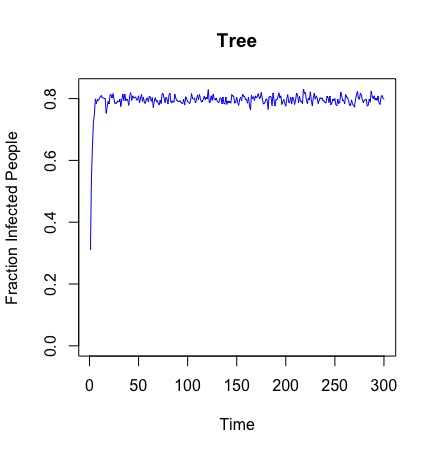
\includegraphics[width=6cm]{tree_4.jpeg}
    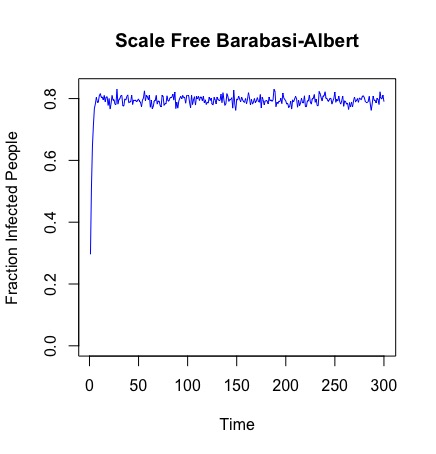
\includegraphics[width=6cm]{barabasi_albert_4.jpeg}
    
\end{center}

\newpage

\subsection{Task 2}

\noindent In this task we are going to try to prove experimentally the theorem (of Charkrabarty) that states:\\

\begin{itemize}
  \item $\frac{\beta}{\gamma} > \frac{1}{\lambda_{1}}$ the epidemic occurs
  \item $\frac{\beta}{\gamma} < \frac{1}{\lambda_{1}}$ the epidemic does not occur\\
\end{itemize}

\noindent where $\lambda_{1}$ is the largest eigenvalue of the underlying contact network.\\

\noindent First we are going to compute $\lambda_{1}$ and then fix values of $\beta$ and $\gamma$ such that the quotient is a little bit above the threshold $\frac{1}{\lambda_{1}}$ and also a little bit bellow $\frac{1}{\lambda_{1}}$.\\

\noindent To define our parameters we print the following table:\\

\begin{center}
 \begin{tabular}{||c c c c||} 
 \hline
 & Low.Beta & High.Beta & Gamma \\ [0.5ex] 
 \hline\hline
 Star & 0.0028 & 0.0035 & 0.1 \\ 
 \hline
 Tree & 0.0332 & 0.0405 & 0.1 \\
 \hline
 Scale Free Barabasi-Albert & 0.0223 & 0.0272 & 0.1 \\
 \hline
 Erdos-Renyi & 0.0018 & 0.0022 & 0.1 \\
 \hline
 Small World - Watts Strogatz & 0.0006 & 0.0007 & 0.1 \\
 \hline
 
 
\end{tabular}
\end{center}

\begin{center}
Table 1: Low Beta and High Beta to define our thresholds.
\end{center}

\noindent In order to prove it we are going to use first the Watts-Strogatz network.\\

\noindent Our threshold is around $0.0065$. So let's select 2 pair of parameters to reproduce the 2 situations:\\

\begin{itemize}
  \item $\beta = 0.0005$ and $\gamma = 0.1$
  \item $\beta = 0.0008$ and $\gamma = 0.1$\\
\end{itemize}

\noindent In the following pictures wee see the difference caused by this small variation of the relation between $\beta$ and $\gamma$. So we can can conclude that the threshold pointed out in the theorem is actually and inflexion point.

\begin{center}
   
    
    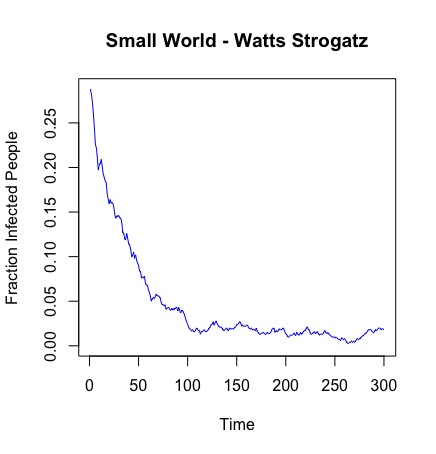
\includegraphics[width=6cm]{watts_strogatz_small.jpeg}
    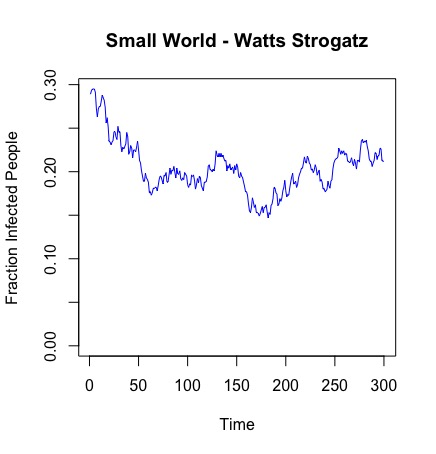
\includegraphics[width=6cm]{watts_strogatz_big.jpeg}
    
    
\end{center}
\newpage

\noindent Now we prove it with the Erdos-Renyi network.\\

\noindent Our threshold is around $0.0020$. So let's select 2 pair of parameters to reproduce the 2 situations:\\

\begin{itemize}
  \item $\beta = 0.0010$ and $\gamma = 0.1$
  \item $\beta = 0.0030$ and $\gamma = 0.1$\\
\end{itemize}


\begin{center}
   
    
    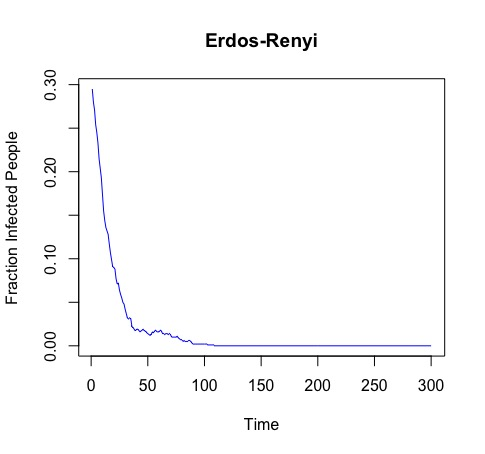
\includegraphics[width=6cm]{erdos_renyi_small.jpeg}
    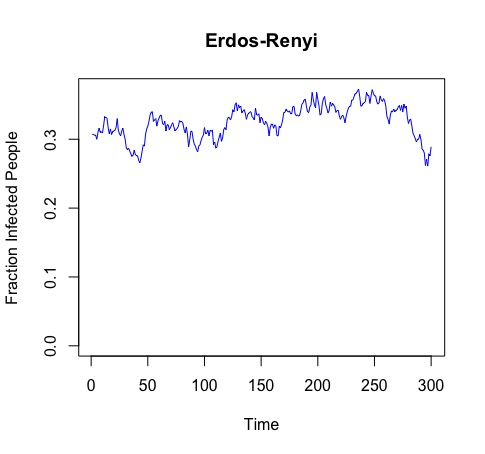
\includegraphics[width=6cm]{erdos_renyi_big.jpeg}
    
    
\end{center}

\newpage
\noindent Now we prove it with the Barabasi-Albert network.\\

\noindent Our threshold is around $0.0250$. So let's select 2 pair of parameters to reproduce the 2 situations:\\

\begin{itemize}
  \item $\beta = 0.0210$ and $\gamma = 0.1$
  \item $\beta = 0.0800$ and $\gamma = 0.1$\\
\end{itemize}


\begin{center}
   
    
    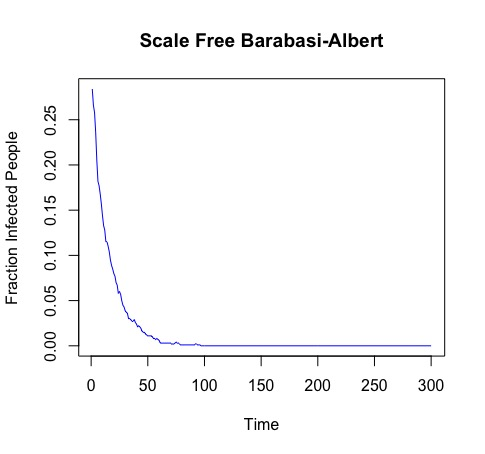
\includegraphics[width=6cm]{barabasi_albert_small.jpeg}
    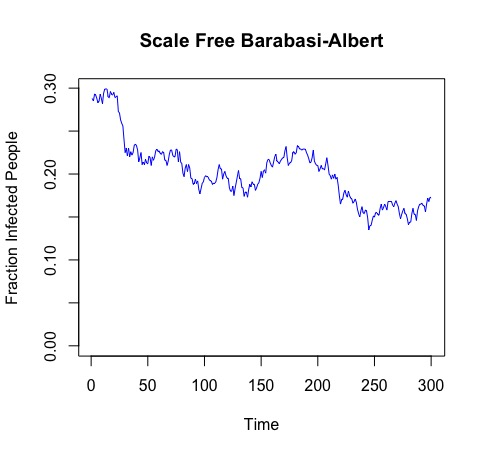
\includegraphics[width=6cm]{barabasi_albert_big.jpeg}
    
    
\end{center}

\noindent We have seen that with the Barabasi-Albert the granularity is not as fine as in the other networks above, and parameters must be fixed a little bit more far away from the threshold.

\newpage

\noindent Now we prove it with the Star network.\\

\noindent Our threshold is around $0.0031$ or $0.0032$. So let's select 2 pair of parameters to reproduce the 2 situations:\\

\begin{itemize}
  \item $\beta = 0.0010$ and $\gamma = 0.1$
  \item $\beta = 0.0080$ and $\gamma = 0.1$\\
\end{itemize}


\begin{center}
   
    
    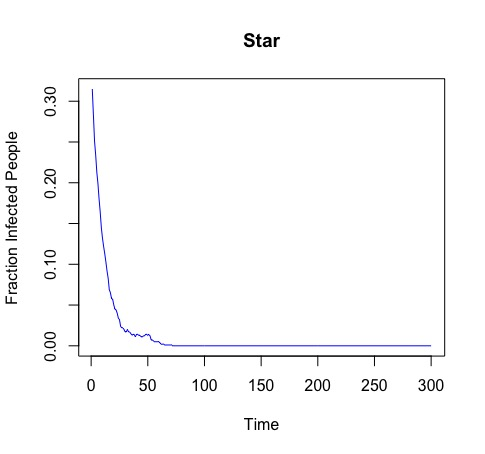
\includegraphics[width=6cm]{star_small.jpeg}
    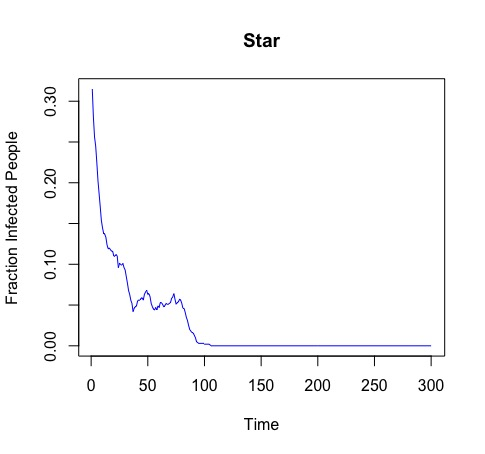
\includegraphics[width=6cm]{star_big.jpeg}
    
    
\end{center}



\newpage




\noindent Finally with the Tree network.\\

\noindent Our threshold is around $0.0360$. So let's select 2 pair of parameters to reproduce the 2 situations:\\

\begin{itemize}
  \item $\beta = 0.0260$ and $\gamma = 0.1$
  \item $\beta = 0.0760$ and $\gamma = 0.1$\\
\end{itemize}


\begin{center}
   
    
    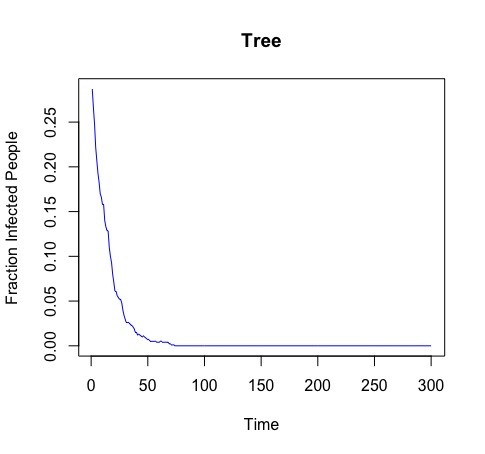
\includegraphics[width=6cm]{tree_small.jpeg}
    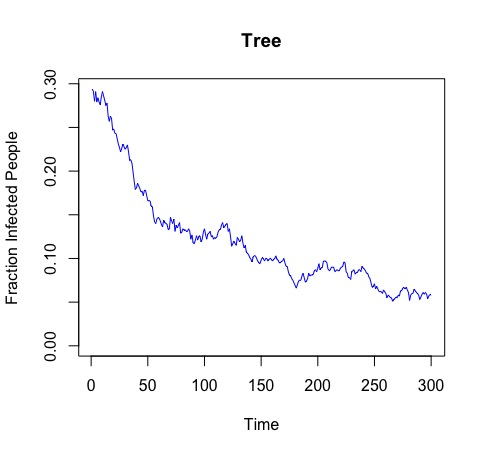
\includegraphics[width=6cm]{tree_big.jpeg}
    
    
\end{center}



\newpage





 

\section{Conclusions}

\noindent In conclusion we can see that $\beta$ and $\gamma$ are determinant parameters in the model but not $p_{0}$.\\

\noindent We can also see that there are networks that model what happens in reality more accurately because the edges between nodes model better relations between people. For example a complete graph does not model at all reality (for that reason was not implemented).\\

\noindent As we know from other labs nodes tend to group themselves in clusters, so it is more likely that the infection is spread in the cluster if one of its members get infected.\\

\noindent We have also seen that there are certain type of networks that are more sensible to the threshold predicted by Charkrabarty than others.\\




\end{document}
